\documentclass[11pt, a4paper]{amsart}
\usepackage{parskip} 
\usepackage{pgfplots}
\usepackage{graphicx}
\title{MAS116/117: Lab 4 Experiments}
\author{Nur Farhazni Najwa Binti Farhan}

\begin{document} 
\maketitle
\section{Graphs created with PGFplots}

\begin{center} %center the graph
\begin{tikzpicture} %will produce normal graph
	\begin{axis}[
		axis lines=center, %the box disappear
		title={$y=\sin (deg(x))$}, %deg(x) function takes a number (in radians) and turns it into the value in degrees; that is, deg(x) = 180x/π
		xlabel=$x$, ylabel=$y$]
	\addplot[smooth, domain=-2*pi:2*pi]{sin(x)};
	\end{axis}
\end{tikzpicture}

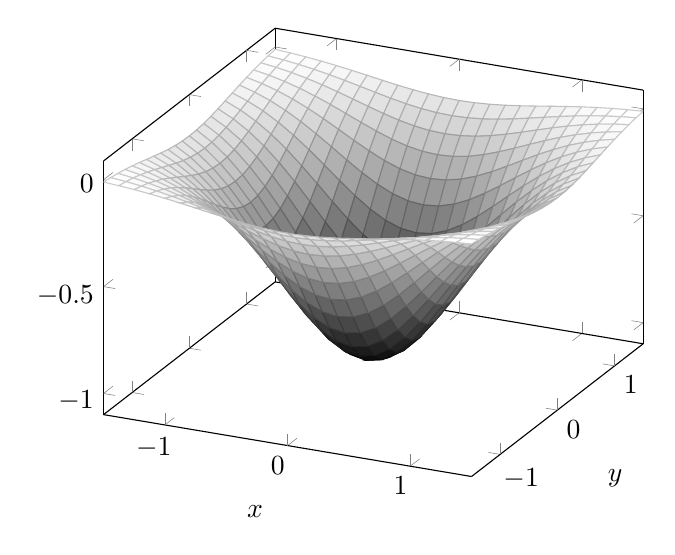
\begin{tikzpicture} %will produce 3d graph
	\begin{axis}[xlabel=$x$, ylabel=$y$, colormap/blackwhite] %put comma, and colormap will produce image in bw
		\addplot3[domain=-1.5:1.5, surf]{-exp(-x^2 - y^2)};
	\end{axis}
\end{tikzpicture}
\end{center}
%more graph : http://pgfplots.sourceforge.net/gallery.html. 

\section{Including image files}
\includegraphics{geogebra_image.pdf} %[scale=0.5] will make the img small, [width=8cm] will make the img smaller %[width=\textwidth] %[width=0.8\textwidth].

Geogebra creates good diagrams; see Figure~\ref{fig:geogebra}
\begin{figure}[tbh]
\includegraphics[width=0.8\textwidth]{geogebra_image.pdf}
\caption{A Geogebra picture}
\label{fig:geogebra}
\end{figure}

\end{document} 

%Homework
\documentclass[11pt, a4paper]{amsart}
\usepackage{parskip} 
\usepackage{pgfplots}
\usepackage{graphicx}
\usepackage{hyperref}
\usepackage{parskip} 
\usepackage{amssymb} 
\usepackage{amsthm} 

\newtheorem{thm}{Theorem}[section]
\newtheorem{lem}[thm]{Lemma}
\newtheorem{defn}[thm]{Definition}

\title{MAS117: Homework 4}
\author{Nur Farhazni Najwa Binti Farhan}

\begin{document} 
\maketitle

\section{Lagrange Interpolation}

\begin{defn}
A quadratic Polynomial is defined as a polynomial of degree $2$, where the highest power of $x$ present in the expression is $x^2$. The general form of a quadratic polynomial is $f(x) = ax^2 + bx + c$, where $a$, $b$, and $c$ are constants and $a \neq 0$. 
\end{defn}

\begin{defn}
For a given points $(x_0, y_0), (x_1, y_1), \dotsb, (x_n,y_n)$, the Lagrange interpolation polynomial $f(x)$ is a polynomial of degree $n$ that passes through each of these points. For three points $(x_0, y_0)$, $(x_1, y_1)$, $(x_2, y_2)$, the polynomial is expressed as:
\[
f(x) := \frac{(x - x_1)(x - x_2)}{(x_0 - x_1)(x_0 - x_2)} y_0 + \frac{(x - x_0)(x - x_2)}{(x_1 - x_0)(x_1 - x_2)} y_1 + \frac{(x - x_0)(x - x_1)}{(x_2 - x_0)(x_2 - x_1)} y_2.
\]
Each term  in the Lagrange interpolation polynomial is called a Lagrange basis polynomial.
\end{defn}

\begin{thm}
if there are $n + 1$ distinct points $(x_0, y_0), (x_1, y_1), \dotsb, (x_n,y_n)$, then the Lagrange interpolation polynomial $P(x)$ is a polynomial of degree at most $n$. 
\end{thm}

\begin{proof}
The Lagrange interpolation polynomial is defined by the formula: 
\[
P(x) = \Sigma_{i=0}^{n} y_i \ell_i(x),
\]
where 
\[
\ell_i(x) = \prod_{\substack{0 \le j \le n \\ j \neq i}} \frac{x - x_j}{x_i - x_j}.
\]
Each $\ell_i(x)$ is a polynomial of degree $n$ since it consists of $n$ linear factors (one for each $x_j$ where $j \neq i$). Therefore, since $P(x)$ is a linear combination of $n + 1$ basis polynomials $\ell_i(x)$, the degree of $P(x)$ is at most $n$. Moreover, if the $y_i$ values are distinct, $P(x)$ will have degree exactly $n$. Thus, we conclude that the Lagrange interpolation polynomial $P(x)$ is a polynomial of degree at most $n$.
\end{proof}

{Sources:}
\begin{itemize}
    \item $https://en.wikipedia.org/wiki/Lagrange_polynomial$
    \item https://mathworld.wolfram.com/LagrangeInterpolatingPolynomial.html
    \item https://brilliant.org/wiki/lagrange-interpolation/
    \item https://www.simplilearn.com/tutorials/statistics-tutorial/lagrange-interpolation
\end{itemize}
\end{document} 
